\documentclass[12pt, a4paper]{ctexart}

\usepackage{amsmath}
\usepackage{array}
\usepackage{appendix}
\usepackage{listings}
\usepackage{xcolor}
\usepackage{fontspec}
\usepackage{underscore}
\usepackage{graphicx}
\setmonofont{Consolas}
\lstset{
	breaklines=true,
	language = C++, 
	numbers=left,
	backgroundcolor=\color{red!0!green!25!blue!25},%代码块背景色为浅灰色
	rulesepcolor= \color{gray}, %代码块边框颜色
	numberstyle= \small,%行号字体
	frame=shadowbox%用方框框住代码块
	frame=single
}

\title{间断有限元第二次作业报告}
\author{九所 $\quad$ 韩若愚}
\date{2022.3.26}
\begin{document}
	\maketitle
	
	\section{题目}
	
	Consider the following linear conservation law:
	\begin{equation}
	\begin{cases}
	&u_t + u_x = 0,\\
	&u(x,0) = u_0(x),
	\end{cases}
	\quad 0 \leq x \leq 1
	\end{equation}
	with periodic boundary condition. Code up the DG scheme for $P^1$ and $ P^2$, together with 2nd order and 3rd order SSP Runge-Kutta method in time, respectively. Use uniform meshes in space and take the final time as $T=2$.
	
	1. Let $u_0(x) = \sin (2 \pi x)$, show error tables of the $L^2$ and $L^\infty$ error.
	
	2. Let
	\begin{equation}
	u_0(x) = 
	\begin{cases}
	&1, \  1/4 \leq x \leq 3/4,\\
	&0, \  elsewhere.
	\end{cases}
	\end{equation}
	
	show pictures of the exact solution and the numerical solution.
	
	\section{算法}
	先对空间进行离散,得到半离散的DG格式。注意到方程中通量函数$f(u) = u$,$f$是$u$的线性函数。
	
	首先对单元$[0,1]$ 进行均匀剖分。假设将区间均匀剖分为$n$份,令:
	\begin{equation}
	0 = x_{\frac{1}{2}} < x_{\frac{3}{2}} < \dots < x_{n-\frac{1}{2}} < x_{n+\frac{1}{2}} = 1
	\end{equation}
	则第$j$个区间为:$ I_j = [x_{j- \frac{1}{2}}, x_{j + \frac{1}{2}}]$,每个区间的长度都为$h = \frac{1}{n}$。记$x_{j+1/2}^- = \lim_{x \in I_j, \, x \to x_{j+1/2}} \, x, \  x_{j+1/2}^+ = \lim_{x \in I_{j+1}, \, x \to x_{j+1/2}} \, x$。
	
	假设对固定的时间t,所求数值解$u_h(\cdot,t)$存在的空间为:$ V_h^k := \{ v : \  v|_{I_j} \in P^k(I_j), j = 1, \dots, n \}$,其中$k$为给定常数,$P^k(I_j)$为定义在$I_j$上的最高次项不超过$k$次的多项式空间,并假设检验函数$v \in V_h^k$,用$v$乘以方程两端并在$I_j$上积分,利用格林公式,并保证$k=0$时算法退化为一阶有限差分格式,于是得到:
	\begin{equation}
	\begin{split}
	&\int_{I_j} (u_h)_t v \, dx - \int_{I_j} u_h v_x \, dx\\
	& \quad + u_h(x_{j+1/2}^-) v(x_{j+1/2}^-) - u_h(x_{j-1/2}^-) v(x_{j-1/2}^+) = 0
	\end{split}
	\label{1}
	\end{equation}
	
	在$I_j$上取定一组$P^k(I_j)$的基底$\{ \phi_j^l \}_{l=0}^k$,则数值解$u_h$在$I_j$上为:$u_h|_{I_j}(x,t) = \sum_{j=1}^n \sum_{l=0}^k \, u_j^l(t) \, \phi_j^l(x)$,求解$u_h$即求解系数$u_j^l, \, j=1, \dots, n, \, l=0, \dots, k$。令检验函数$v = \phi_j^m, \, m=0, \dots, k$,则方程组(\ref{1})变为:
	\begin{equation}
	\begin{split}
	& \sum_{l=0}^k (\int_{I_j} \phi_j^l(x) \phi_j^m(x) \, dx ) \frac{d}{dt} u_j^l(t) = \\
	&\quad  \sum_{l=0}^k (\int_{I_j} \phi_j^l(x) (\phi_j^m(x))_x \, dx - \phi_j^l(x_{j+1/2}) \phi_j^m(x_{j+1/2}) ) u_j^l(t)\\
	& \quad  - u_h(x_{j-1/2}^-) \phi_j^m(x_{j-1/2}) 
	\end{split}
	\label{2}
	\end{equation}
	
	为便于求解,假设参考单元$I = [-1,1]$,对每个单元$I_j$都有一个到$I$的微分同胚$\Phi_j : I_j \to I$,$ \xi := \Phi_j(x) = \frac{2}{h} (x - x_{j-1/2}) - 1$。在参考单元上取定一组$P^k(I)$的基底$\{\phi^l\}_{l=0}^k$,则由$\Phi_j$将$\phi^l$拉回到$I_j$上得到的函数组$\{(\Phi_j^{-1})^* \phi^l\}$也是$P^k(I_j)$的基底,不妨就设为$\{\phi_j^l\}$。于是每个单元$I_j$上的计算都可以在$I$上进行,方程组(\ref{2})变为:
	\begin{equation}
	\begin{split}
	& \frac{h}{2} \sum_{l=0}^k (\int_{I} \phi^l \phi^m \, d\xi) \cdot \frac{d}{dt} u_j^l(t) = \\
	& \quad \sum_{l=0}^k (\int_{I} \phi^l (\phi^m)_{\xi} \, d\xi - \phi^l(1) \phi^m(1)) u_j^l(t)\\
	& \quad + u_{j-1/2}^- \phi^m(-1)
	\end{split}
	\label{3}
	\end{equation}
	上式可以写成方程组的形式:
	$$
	A \frac{d}{dt} \vec{u}_j = B \vec{u}_j + u_{j-1/2}^- \cdot C
	$$
	\begin{equation}
	\frac{d}{dt} \vec{u}_j =A^{-1} (B \vec{u}_j + u_{j-1/2}^- \cdot C) := F_j(\vec{u}_j), \quad j = 1,2, \dots,n
	\label{4}
	\end{equation}
	这是一个关于向量$\vec{u}_j$的常微分方程组,其中$u_{j-1/2}^- = \sum_{l=0}^k u_{j-1}^l \phi_j^l(x_j-1/2) =  \sum_{l=0}^k u_{j-1}^l \phi^l(1) $$, \  j= 1,2, \dots,n$,其中$j$是循环指标,$j=0$时$j-1 = n$。
	
	为了求解(\ref{4}),当$k>0$时,一般的欧拉前插方法不稳定。需要使用Runge-Kutta法对方程组进行离散,同时保证稳定性。对方程$u_t = F(u)$的$s$阶RK法的Shu-Osher形式写为:
	\begin{equation}
	\begin{split}
	& u^{(0)} = u^n \\
	& u^{(i)} = \sum_{l=0}^{i-1} \alpha_{il} u^{(l)} + \Delta t \beta_{il} F(u^{(l)}), \  i = 1,2,\dots,s\\
	& u^{n+1} = u^{(s)}\\
	& \alpha_{il} , \beta_{il} \ge 0, \quad \sum_{l=0}^{i-1} \alpha_{il} = 1, \  i = 1,2,\dots,s
	\end{split}
	\end{equation}
	
	SSPRK(2,2)和SSPRK(3,3)格式分别如下:
	\begin{align*}
	&SSPRK(2,2):\\
	& \quad u^{(0)} = u^n\\
	& \quad u^{(1)} = u^{(0)} + \Delta t F(u^{(0)})\\
	& \quad u^{n+1} = \frac{1}{2} u^{(0)} + \frac{1}{2} u^{(1)} + \frac{1}{2} \Delta t F(u^{(1)})\\
	&\\
	&SSPRK(3,3):\\
	& \quad u^{(0)} = u^n\\
	& \quad u^{(1)} = u^{(0)} + \Delta t F(u^{(0)})\\
	& \quad u^{(2)} = \frac{3}{4} u^{(0)} + \frac{1}{4} u^{(1)} + \frac{1}{4} \Delta t F(u^{(1)}) \\
	& \quad u^{n+1} = \frac{1}{3} u^{(0)} + \frac{2}{3} u^{(2)} + \frac{2}{3} \Delta t F(u^{(2)})
	\end{align*}
	
	同时为保证稳定性,对时间步长$\Delta t$的选取还要满足CFL条件。
	
	
	\section{计算结果}
	
	为了方便计算,取$P^k(I)$上的基函数为Legendre函数。为了满足CFL条件,将时间步长$\Delta t$取为$h/5$。算法使用C++实现。
	
	当初值为$u_0(x)= \sin 2 \pi x$时,在终止时刻$t=2$时计算真解与数值解的$L^2$范数和$L^\infty$范数误差。$P^1,P^2$元的误差表如下(保留三位小数):
	\begin{table}[htbp]
		\centering
		\caption{$P^1$}
		\begin{tabular}{| p{40pt}<{\centering} | p{80pt}<{\centering} | p{60pt}<{\centering} || p{80pt}<{\centering} | p{60pt}<{\centering}|}
			\hline
			n & $L^2$ error & order & $L^\infty$error & order\\
			\hline
			10 & 3.270e-2 & & 5.807e-2 & \\
			\hline
			20 & 8.303e-3 & 1.978 & 1.262e-2 & 2.202\\
			\hline
			40 & 2.257e-3 & 1.879 & 3.891e-3 & 1.697\\
			\hline
			80 & 5.952e-4 & 1.923 & 1.062e-3 & 1.873\\
			\hline
			160 & 1.531e-4 & 1.959 & 2.767e-4 & 1.940\\
			\hline
			320 & 3.884e-5 & 1.979 & 7.054e-5 & 1.972\\
			\hline
		\end{tabular}
	\end{table}

\begin{table}[htbp]
	\centering
	\caption{$P^2$}
	\begin{tabular}{| p{40pt}<{\centering} | p{80pt}<{\centering} | p{60pt}<{\centering} || p{80pt}<{\centering} | p{60pt}<{\centering}|}
		\hline
		n & $L^2$ error & order & $L^\infty$error & order\\
		\hline
		10 & 2.073e-3 & & 3.955e-3 & \\
		\hline
		20 & 2.665e-4 & 2.960 & 5.142e-4 & 2.943\\
		\hline
		40 & 3.378e-5 & 2.980 & 6.553e-5 & 2.972\\
		\hline
		80 & 4.254e-6 & 2.989 & 8.254e-6 & 2.989\\
		\hline
		160 & 5.342e-7 & 2.993 & 1.067e-6 & 2.952\\
		\hline
		320 & 6.735e-8 & 2.988 & 1.822e-7 & 2.550\\
		\hline
	\end{tabular}
\end{table}

	当初值为$u_0(x) = \begin{cases} 1, \  1/4 \leq x \leq 3/4,\\ 0, \ elsewhere\end{cases}$时,终止时刻$t=2$时取空间步长$h = 0.01$,$P^1, \  P^2$元求解得到的数值解$u\_h$和真解$u$图像如下:

\begin{figure}[htbp]
	\centering
	\caption{$P^1$}
	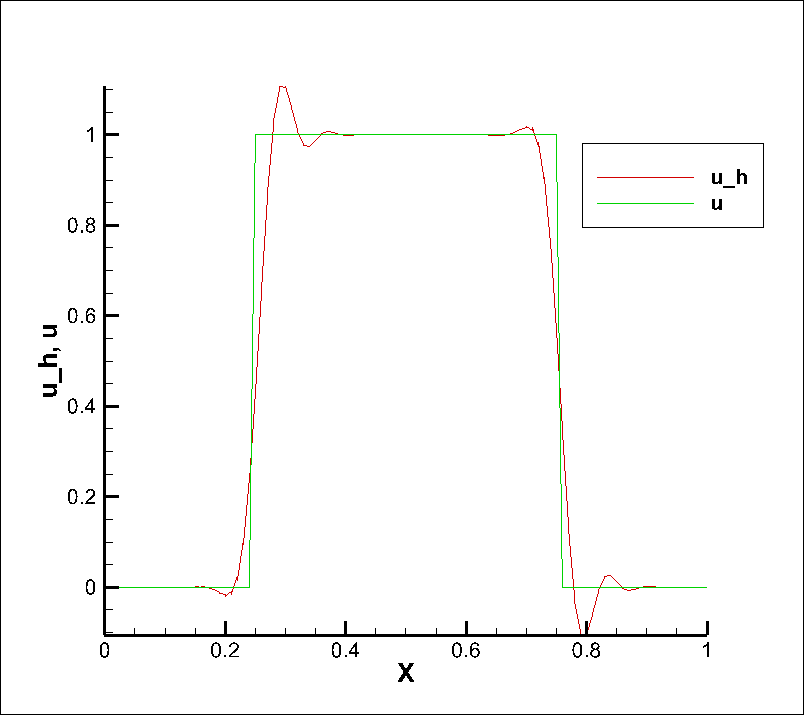
\includegraphics[width=15cm]{P1.png}
\end{figure} 
\begin{figure}[htbp]
	\centering
	\caption{$P^2$}
	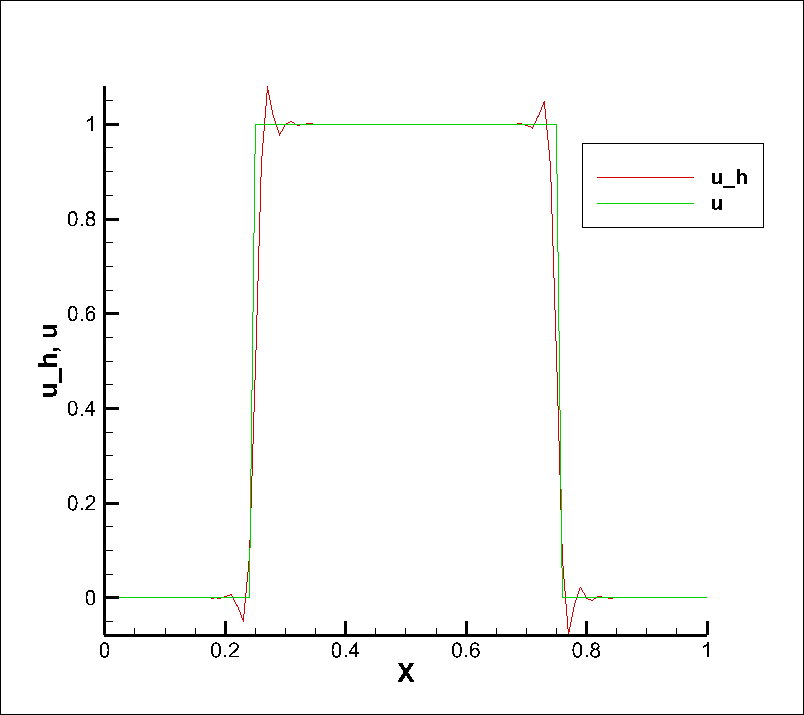
\includegraphics[width=15cm]{P2.png}
\end{figure} 
	
	\section{分析}
	
	可以看到在本例中,当步长$\Delta t = h/5$时,$P^1$元和$P^2$元在$L^2, \  L^\infty$下的收敛阶分别在2和3左右。但是当划分个数在320时,$P^2$元$L^\infty$下的收敛阶出现了问题。在上一次的作业中也是在划分等于320时出现了类似问题。我觉得这可能不是我的代码有错误,目前关于问题的根源我还没有头绪。
	
	在初值有间断的情况下,计算得到的数值解在间断出出现了一些剧烈的波动,这是由于方程只存在弱解造成的,要避免这种情况可以在方程中添加人工粘性项。另外我想到在图像处理中经常会用到滤波函数过滤图像中的高频部分,如果对数值解进行类似的操作限制$u_x,\  u_{xx}$的大小应该也能让解的图像看起来更平滑,不过这种操作本质上应该和添加人工粘性项相同。
\end{document}